\setcounter{chapter}{+2}

\section{Informações Técnicas}
Rodamos os algoritmos anteriormente apresentados, e vamos mostrar os resultados obtidos. Sobre a máquina:
\newline

\textbf{Disco Rígido:} Seagate ST1000DM003-1ER162 7200rpm;
\par
\textbf{Processador:} Intel Core i7-4790K CPU @ 4.00Ghz;
\par
\textbf{Memória:} 8,00 GB 1600Mhz;
\par
\textbf{Sistema Operacional:} Windows 8.1 Pro;
\newline

Sobre o arquivo a ser ordenado e o algoritmo:
\par
\textbf{Estrutura utilizada:} Estrutura denominada medição, contendo índice, temperatura variando de 0 a 50 graus, dia, mês, ano, sendo todos os campos do tipo long long (8 bytes);
\par
\textbf{Tamanho de cada medição:} 40 bytes; 
\par
 
\textbf{Quantidade de medições:} 322.122,547;
\par

\textbf{Tamanho total do arquivo:} 12,0 GB = 12.884.901.888 bytes;
\par
\textbf{Linguagem em que o algoritmo foi escrito:} Linguagem C;
\par
\textbf{Forma de ordenação:} Crescente, ordenando a temperatura;
\newpage

\section{Resultados}

\textbf{Tempo para gerar o arquivo inicial em média:} 98 segundos;
\par

\begin{figure}[h]
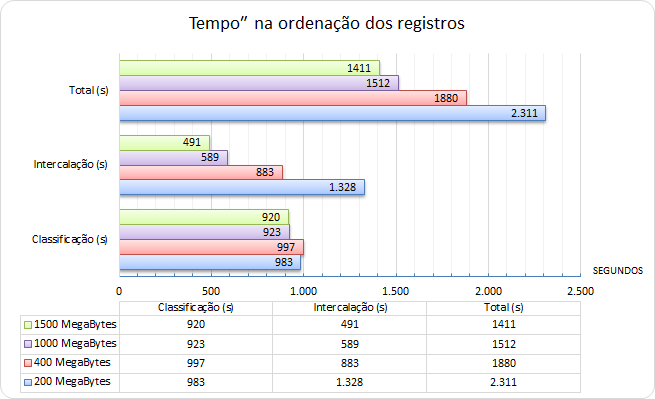
\includegraphics[width=.7\paperwidth]{tempoOrdenacaoRegistros}
\caption{Tempo para Ordenar 12GB dividindo em blocos de N MegaBytes carregados na memória.}
\label{fig:tempoOrdenacaoRegistros}
\end{figure}
Obs.: Esses valores são aproximações.


\subsection{Análise dos Resultados}
\par
No gráfico acima, tem-se os resultados dos experimentos realizados em cima do algorítmo de ordenação. Temos três grandes sessões, uma mostrando o tempo total do algorítmo, uma mostrando somente o tempo necessário para a etapa da intercalação e por fim, a ultima sessão mostra o tempo de classificação. Os testes foram realizados alterando o tamanho do bloco carregado na memória (1500, 1000, 400 e 200 MegaBytes) em um deteminado instante e o tempo foi medido em segundos.
\par
\textbf{Tempo de intercalação:} Aqui nota-se uma discrepância nos tempos de cada bloco. O maior bloco, 1500 MB, realizou a operação de intercalação em aproximadamente 8 minutos, ja quando carregamos apenas um bloco de 200 MB, seu tempo subiu para 22 minutos. Isso ocorre devido ao fato de que, quando um bloco maior é carregado na memória, este gera menos arquivos na etapa de classificação, logo, o Sistema Operacional realiza menos operações para abrir e fechar arquivos, ocasionando num tempo total muito menor.
\par
\textbf{Tempo de classificação:} Na classificação, o tempo se manteve estável e não se diferenciou muito com o aumento dos blocos. Embora ele necessite criar menos arquivos quando há um bloco maior na memória, ainda assim, ele trabalha com menos blocos que a etapa de intercalação.
\par
Para se ter um desempenho maior no algorítmo, um maior bloco deve ser utilizado em sua execução visando a criação da menor quantidade de arquivos possíveis. É necessário ter um cuidado especial na seleção do bloco, pois precisa-se levar em consideração a quantidade máxima de memória que o sistema operaciona consegue ceder sem que ele mesmo seja prejudicado devido a swap e outros fatores.